\documentclass[tikz,border=3.14pt]{standalone}
\makeatletter
\tikzset{%
  rel/.code={%
    \pgfsetlinetofirstplotpoint%
    \edef\rel@curr@x{\the\tikz@lastx}%
    \edef\rel@curr@y{\the\tikz@lasty}%
    \let\rel@plot\tikz@@@plot
    \def\tikz@@@plot{%
      \let\rel@streampoint\pgfplotstreampoint
      \def\pgfplotstreampoint####1{%
        \pgf@process{####1}%
        \advance\pgf@x by \rel@curr@x\relax
        \advance\pgf@y by \rel@curr@y\relax
        \edef\rel@point{\noexpand\rel@streampoint{\noexpand\pgfqpoint{\the\pgf@x}{\the\pgf@y}}}%
        \rel@point
      }%
      \rel@plot
    }%
  }%
}%
\makeatother
\begin{document}
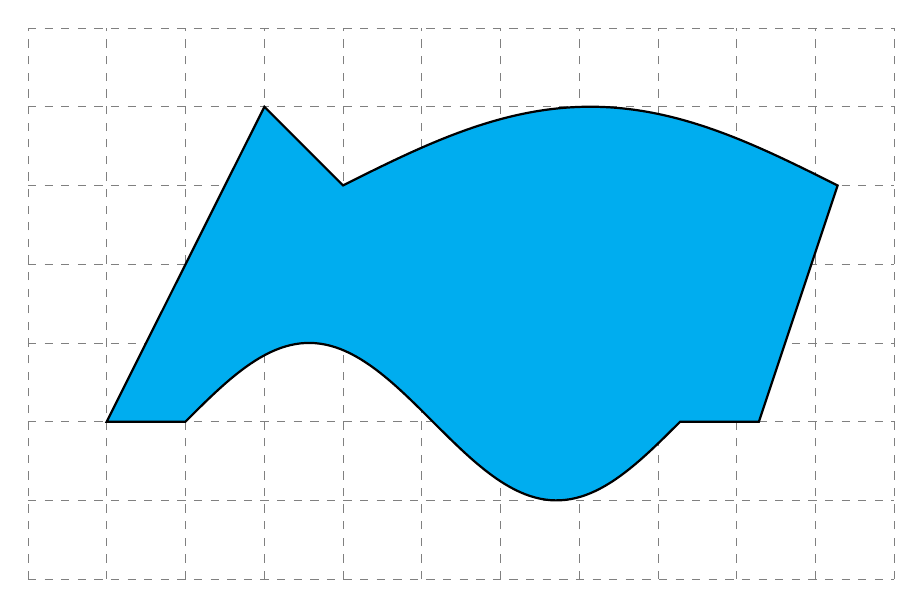
\begin{tikzpicture}[trig format=rad]
\draw[help lines,dashed] (-1,-1) grid (10,6);
\draw[thick,fill=cyan]
    (0,1) -- ++(1,0) 
    plot[rel,domain=0:2*pi,samples=100] (\x,{sin(\x)}) --
    ++(1,0) --
    ++(1,3) --
    plot[rel,domain=0:pi,samples=100] (-2*\x,{sin(\x)})
    plot[rel,domain=0:1,samples=100] (-\x,\x) 
    -- cycle
;
\end{tikzpicture}
\end{document}
